% !TeX spellcheck = en_US
\documentclass[french]{yLectureNote}

\title{Séries - Analyse 2}
\subtitle{Chimie}
\author{Paulhenry Saux}
\date{\today}
\yLanguage{Français}

\professor{IHallery}%isabelle.hallery@univ-tlse3.fr
\usepackage{graphicx}%----pour mettre des images
\usepackage[utf8]{inputenc}%---encodage
\usepackage{geometry}%---pour modifier les tailles et mettre a4paper
%\usepackage{awesomebox}%---pour les boites d'exercices, de pbq et de croquis ---d\'esactiv\'e pour les TP de PC
\usepackage{tikz}%---pour deiffner + d\'ependance de chemfig
\usepackage{tkz-tab}
\usepackage{chemfig}%---pour deiffner formules chimiques
\usepackage{chemformula}%---pour les formules chimiques en \'equation : \ch{...}
\usepackage{tabularx}%---pour dimensionner automatiquement les tableaux avec variable X
\usepackage{awesomebox}%---Pour les boites info, danger et autres
\usepackage{menukeys}%---Pour deiffner les touches de Calculatrice
\usepackage{fancyhdr}%---pour les en-t\^ete personnalis\'ees
\usepackage{blindtext}%---pour les liens
\usepackage{hyperref}%---pour les liens (\`a mettre en dernier)
\usepackage{caption}%---pour la francisation de la l\'egende table vers Tableau
\usepackage{pifont}
\usepackage{array}%---pour les tableaux
\usepackage{lipsum}
\usepackage{yFlatTable}
\usepackage{multicol}
\newcommand{\Lim}[1]{\lim\limits_{\substack{#1}}\:}
\renewcommand{\vec}{\overrightarrow}
\newcommand{\N}[0]{\mathbb{N}}
\begin{document}
\setcounter{chapter}{0}
\chapter{Oscilloscope }
\section{Composantes du signal}
On peut séparer le signal en 2 parties :
\begin{itemize}
 \item Une partie alternative, dont la moyenne est nulle
 \item Une partie continue, appellée aussi offset
\end{itemize}
L'Oscilloscope possède 2 modes :
\begin{itemize}
 \item Le mode AC (Alternative Current) qui affiche seulement la partie variable (ou alternative) du courrant
 \item Le mode DC (Direct Current) qui affiche les 2 composantes (Offset + partie variable)
\end{itemize}
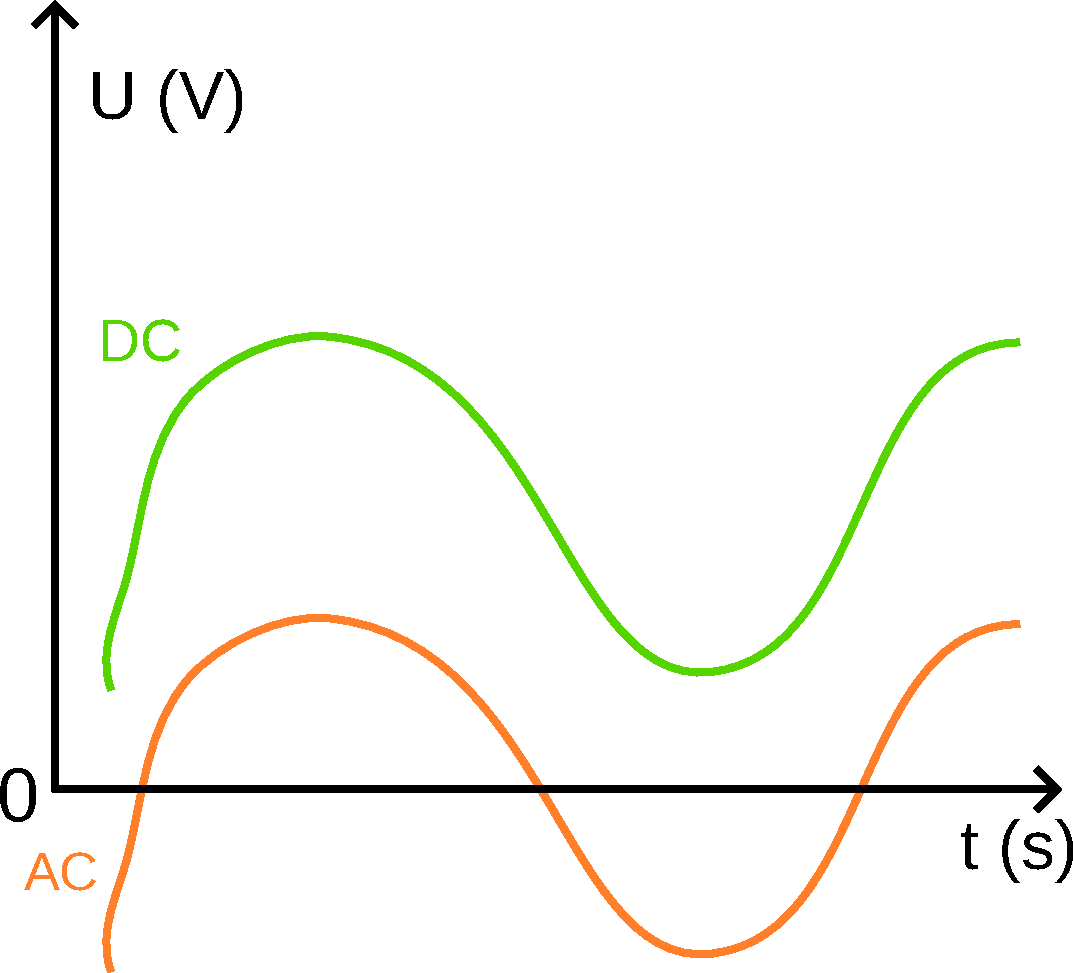
\includegraphics[scale=0.5]{path1}

Ainsi, lorsque l'on sélectionne AC, on applique un filtrage au signal pour ne garder que la partie alternative et enlever la partie continue. La partie continue a une période qui tend vers l'infini, donc une fréquence qui tend vers 0. On applique donc un filtre passe-haut  avec une fréquence de coupure de l'ordre du Hz.
\section{Mesure d'un décalage de phase}
 \begin{theorem}[Formule du décalage de phase]
  On utilise \(\varphi = \pm \frac{d}{D}\) avec \(d\) la distance la plus petite séparant les 2 courbes et \(D\) la période de la courbe de référence.
 \end{theorem}
Si v1 passe
par 0 avec une pente de signe donné à l'instant to , v2 passe par 0 avec la même pente à l'instant to - τ.
Si τ est positif, v2 est en avance sur v1 et \(\varphi\) est positif. Dans le cas contraire c'est v1 qui est en avance sur v2.

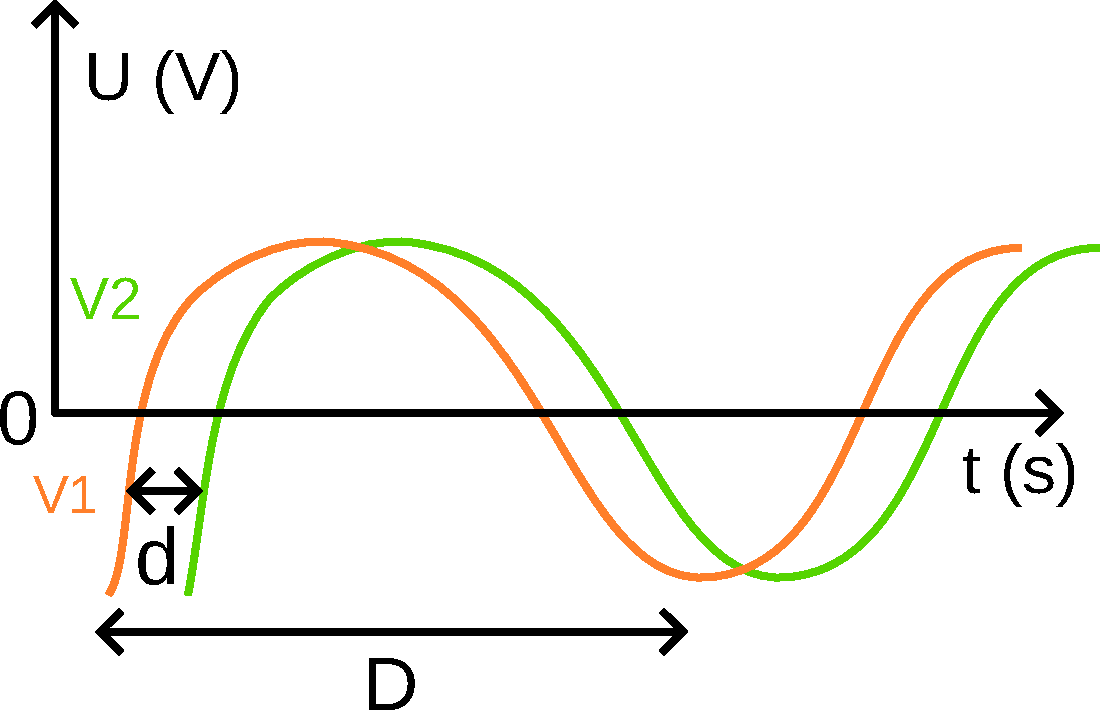
\includegraphics[scale=0.5]{path2}
\end{document}

